 \documentclass[11pt]{report}
  \usepackage{color}
  \usepackage{geometry}
  \usepackage{enumitem}
  \usepackage{mathtools}
  \usepackage{ragged2e}
  \usepackage{listings}
  \usepackage{graphicx}
  \geometry{%
  a4paper,%
  top=2.5cm,%
  bottom=2.5cm,%
  left=2.5cm,%
  right=2.5cm%
}

\begin{document}


\chapter{Cell and their normal functions}
\section{\color{red}Cell as signal analysis device}
\emph{For Biologist :} The cell is the basic structural, functional and biological unit of all known living organisms \cite{wiki:cell}.
\subsection{\color{blue}Cellular Organization}
\subsubsection{Context 1}
Each cell is surrounded by the Extracellular Matrix (ECM) which is a collection of extracellular molecules secreted by the cells that provides structural and biochemical support to the surrounding cells \cite{wiki:ecm}.
Blood cells are such type of cells.
The major structural proteins of the extracellular matrix are members of the large collagen protein family. Collagens form the fibrils that characterize the extracellular matrix of connective tissues, as well as forming networks in basal laminae.

\subsubsection{Context 2}
A group of cells are surrounded by the Extracellular Matrix (ECM).
Skin cells are such type of cells.

\section{\color{red}Concepts of proteins and their role in biological systems}
\subsection{\color{blue}Inside Cells}
\subsubsection{Protein :}
The primary responsibility of proteins is to execute the tasks directed by that information \cite{cooper2007cell}.
Proteins are the most diverse of all macromolecules, and each cell contains several thousand different proteins, which perform a wide variety of functions.
The roles of proteins include serving as structural components of cells and tissues, acting in the transport and storage of small molecules (e.g., the transport of oxygen by hemoglobin), transmitting information between cells (e.g., protein hormones), and providing a defense against infection (e.g., antibodies).
The most fundamental property of proteins, however, is their ability to act as enzymes, which catalyze nearly all the chemical reactions in biological systems.

Ligands and Receptors are also proteins.

Protiens are 'polymers' like molecules which are well structured.
Protiens dictates many aspects of biological systems including signal processing.

Every protein is produced after processing of some gene.
DNA -> RNA -> Protein

\section{\color{red}Level of signal processing in biological cells}
Following are the various levels of signal processing :
\begin{enumerate}
 \item Extracellular level signaling
 \item Cell surface level signaling
 \item Intracellular level signaling
\end{enumerate}

 \chapter{Stem Cells and their role in our body}
 \section{\color{red}Difference between normal cells and stem cells}
 Stem cells differ from normal cells in the following ways \cite{hall1989stem}:
 \begin{itemize}
  \item During the lifespan of an organism, stem cells have unlimited self renewal capacity.
  \item Stem cells can undergo asymmetric cell divisions, i.e., one daughter is itself a stem cell while the other daughter will
  eventually differentiate terminally.
  \item The process of asymmetric division is irreversible as daughters committed to undergo terminal differentiation are not stem
  cells.
 \end{itemize}
 Also the property of \textbf{stemness} allows stem cells to modify their internal signal processing mechanism significantly.
 
 \section{\color{red}The role of stem cells in our body and their working}
 Stem cells are found in many regions of our body like brain, liver \cite{Watt2000}, bone marrow, epidermis, intenstinal epithelium \cite{hall1989stem}, etc..
 Cell divisions have different contributions during embryonic development and during adult life. During embryonic development, cell
 divisions produce new differentiated cells and increase the total number of cells while during adult life, cell divisions maintain the number of differentiated cells
 at a constant level. In tissues with permanently renewing populations like blood, testis, the terminally differentiated cells have
 a very short life span. They are replaced through proliferation of stem cells\cite{hall1989stem}. Stem cells also help in tissue repair by producing
 new cells rapidly.

 \section{\color{red}Life cycle of a stem cell}
 Stem cells have self renewal property and they can either divide Symmetrically or Asymmetrically(Discussed later). A Parent cell
 can either divide into two daughter stem cells or a daughter stem cell and one Transit Amplifying cell Which will eventually differentiate
 terminally.
 
 i.e. 
 
  Parent Cell $\xrightarrow{Symmetric Division}$ [Daughter Stem Cell 1] + [Daughter Stem Cell 2]
  
  \begin{center}
    OR
  \end{center}

  Parent Cell $\xrightarrow{Asymmetric Division}$ [Daughter Stem Cell] + [Transit Amplifying Cell]
  
  \chapter{Differentiation of Stem Cells}
  
  \section{\color{red}Meaning of stem cell differentiation}
  Through the process of cellular differentiation, a less specialized cell turns into a more specialized cell type(Wiki). It can also
  be defined as a qualitative change in the cellular phenotype as a result of the the onset of synthesis of new gene products. A
  cell  can undergo many differentiations during its life. A cell can be differentiated with respect to another cell only as the
  process of differentiation is qualitative\cite{hall1989stem}. For e.g.- A stem cell can differentiate into a brain cell eventually.
  
  
  \section{\color{red}Types of stem cell differentiation}
  There are two types of stem cell differentiation:\\ 
  \begin{enumerate}
   \item \textbf{Natural Pluripotent}: Natural Pluripotent Stem cells have the potential to differentiate into any of the three germ layers: endoderm, mesoderm or ectoderm
   \item \textbf{Induced Pluripotent}: Induced Pluripotent Stem Cells (IPS cells or IPSCs) are a type of Pluripotent stem cells that are artificially derived from non-pluripotent stem cells, by  inducing forced expression of certain genes and transcription factors.

  \end{enumerate}
  
  \chapter{Code structure}
   \section{\color{red} Components of a System}
  The simulation environment consist of the following components:
  \begin{itemize}
   \item Stem Cells
   \item Transit Amplifying Cells
   \item Normal Cells
   \item ECM fibers
  \end{itemize}
  
  \section{\color{red} Operations done by simulation class}
  The following operations are supported
  \subsection{\color{blue}Move Cells}
  This function determines the next location for each cell to move to using Gaussian Probability. It calculates the 
  total number of fibers in the neighbourhood and then uses it to calculate probabilty.
  \subsection{\color{blue}Update E Cadherin - $ \beta $ Catenin value}
  This function updates the E Cadherin - $ \beta $ Catenin value based on the following logic:
  \begin{itemize}
   \item Calculate the total ECadherin value by summing the ECadherin value of all the neighbours.
   \item Use the following formula to update the ECadherin- $\beta$ Catenin value:\\
   \begin{equation}
    EB = \frac{1}{2}\bigg(\frac{k}{sumFiber+k}*EB + \frac{totalNeigbourEC}{N}\bigg)
   \end{equation}
   where
   \begin{description}[labelindent=2cm]
    \item \textbf{sumFiber} = The sum of the fiber counts of the neighbours
    \item \textbf{k} = A constant
    \item \textbf{totalNeighbourEC} = total E Cadherin value
    \item \textbf{N} = Number of neighbours
    \end{description}
   \end{itemize}
   \subsection{\color{blue}Evolve genetic code}
   Performs following computations: 
   \begin{itemize}
    \item STAT3 	= 	LIF
    \item TCF3 		= 	CH' . MEK{\_}ERK'
    \item MEK{\_}ERK 	= 	PD'
    \item GBX2		=	STAT3
    \item KLF4		=	STAT3 . GBX2
    \item TFCP2L1	=	ESMB . TCF3' . STAT3 . KLF4 . OCT4'
    \item ESMB		=	TFCP2L1 . TCF3' . NANOG
    \item OCT4		=	SOX2 . KLF2 . ESMB'
    \item SOX2		=	SALL4 . NANOG
    \item NANOG		=	MEK{\_}ERK' . OCT4 . KLF2
    \item KLF2		=	KLF4 . SALL4
    \item SALL4		=	TFCP2L1
   \end{itemize}

  \subsection{\color{blue}Increase age of cells}
  This function increases the age of all cells by 1 and splits(divides) a cell into two if its age becomes more than 30.
  The location of the new cell is determined using Gaussian probabilty concept as used in moving cells.

  \section{\color{red} Operations done by cell class}
  The following operations are supported
  \subsection{\color{blue}Increase cell age}
  This function increases the age of cell by 1.
  \subsection{\color{blue}Determination of favorable location}
  This function identifies a location in the neighbourhood of the given cell(i.e. within its sensing radius)  where that cell can be moved or a new daughter cell can be added. The probability of selecting a location is defined by the Gaussian probability distribution.
  Thus, it is called before adding a new daughter cell or moving the given cell.
  For this operation we have assumed that every cell has a centroid associated with it. So, while initializing the cell, we select a random lattice point (where no cell or ECM fiber is present) as the centroid of that cell.
  \subsection{\color{blue}Cell Division}
  This function divide the cells (normal cells) and position the new cells at favourable location.
  
  \section{\color{red} Operations done by AutomatonCell class}
  The following operations are supported
  \subsection{\color{blue}Increase number of fibers at that point}
  This function increases number of fibers at that particular point by 1.
  
  \section{\color{red} Operations done by Utilities class}
  The following operations are supported
  \subsection{\color{blue}Generate output ECM file}
  This function writes the state of lattice (Environment) in file "ptMap.xyz" in following format : \\
  \begin{itemize}
    \item First line specifies the number of points in the xyz file.
    \item Second line is a comment line
    \item Remaining lines specifies each point (record) in format : \\
    $<cell Type> <x Dimension> <y Dimension> <z Dimension> <cell Count>$
   \end{itemize}
   \subsection{\color{blue}Write current state/iteration}
   This function writes the state/iteration changes of lattice (Environment) in a file named "$<iterationNumber>$.txt" in the following format :
   \begin{itemize}
    \item For each point in the lattice, following values are specified \\
    $<x Dimension>,<y Dimension>,<z Dimension>,<cell Type>,<cell Id>,<cell Age>$ \\ \\
    Note : cell age is -1 for empty (free) points 
   \end{itemize}
   
  \section{\color{red} Operations done by Environment class}
  The following operations are supported
  \subsection{\color{blue}Setting up Extra Cellular Matrix}
  This function initializes the simulation environment with the given number of ECM (Extra-Cellular Matrix) fibers (as specified in the configuration file), position them at random locations with random orientations in the environment (lattice).
  For each point within the environment, it also calculates the number of fibers intersecting at that point.
  \subsection{\color{blue}Initialization of cells}
  This function initializes the attributes of every cell with default values and assign a unique ID to each cell.
  
  \section{\color{red} Operations done by SimulationParameters class}
  The following operations are supported
  \subsection{\color{blue}Loading Simulation Parameters}
  This function loads the simulation parameters from the configuration file (uscp.conf).
  
  \section{\color{red} Operations done by StemCell class}
  The following operations are supported
  \subsection{\color{blue}Symmetric Division}
  This function divides the stem cell symmetrically, i.e. the parent stem cell is divided into two stem cells.
  \subsection{\color{blue}Asymmetric Division}
  This function divides the stem cell asymmetrically, i.e. the parent stem cell is divided into a stem cell and a transit-amplifying cell.
  
  \chapter{Implementation}
  \section{\color{red}Classes}
  \subsection{\color{blue}AutomatonCell}
  \paragraph{Description}
  Class representing a Lattice Point
  \subsection{\color{blue}Cell}
  \paragraph{Description}
  Class representing a cell
  \subsection{\color{blue}Environment}
  \paragraph{Description}
  This class provides functions for setting up the simulation environment
  \subsection{\color{blue}Line}
  \paragraph{Description}
  Class representing a line in 3d plane
  \subsection{\color{blue}Point}
  \paragraph{Description}
  Class representing a 3 dimensional point
  \subsection{\color{blue}Simulation}
  \paragraph{Description}
  This class provides necessary functions for performing the simulation
  \subsection{\color{blue}SimulationParameters}
  \paragraph{Description}
  Class for loading simulation parameters
  \subsection{\color{blue}StemCell}
  \paragraph{Description}
  This class models the Stem Cells and is derived from the Cell class
  \subsection{\color{blue}TACell}
  \paragraph{Description}
  This class models the Transit Amplifying Cells and is derived from the Cell class
  \subsection{\color{blue}Utilities}
  \paragraph{Description}
  Class for generating the Output
  \subsection{\color{blue}Var}
  \paragraph{Description}
  Class representing a coordinate variable
  \pagebreak
  \section{\color{red}Class Diagram}
    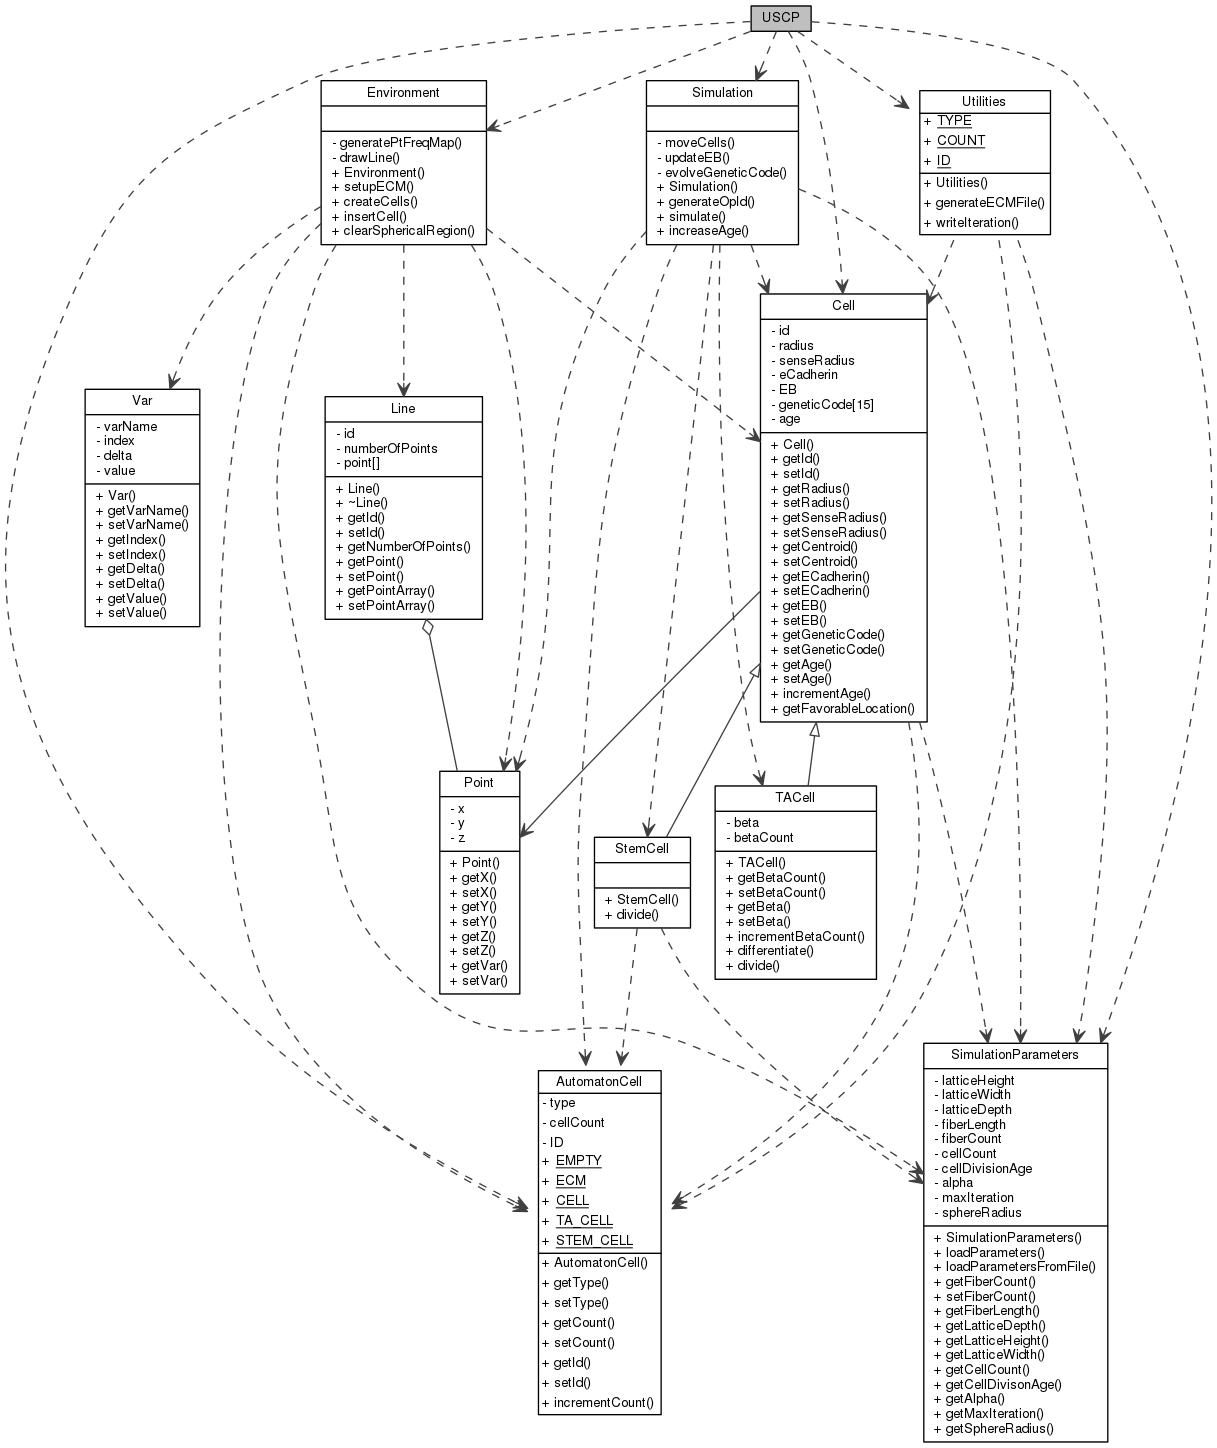
\includegraphics[width=7in]{../diag/classDiagram/class_diag.png}
  
  \section{\color{red}Description of Configuration Files}
  \subsection{\color{blue}"uscp.conf"}
  \subsubsection{\color{green}Description: }
  The structure of uscp.conf is as follows:
  \begin{itemize}
   \item \textbf{Parameters} : The root of xml file.
   \begin{itemize}
    \item \textbf{Lattice} : Represents the simulation environment.
    \begin{itemize}
     \item \textbf{Height} : The Height of the lattice.
     \item \textbf{Width} : The Width of the lattice.
     \item \textbf{Depth} : The Depth of the lattice.
    \end{itemize}

    \item \textbf{FiberCount}: The number of fibres in the lattice.
    \item \textbf{FiberLength} : The Length of each fibre.
    \item \textbf{CellCount} : The number of normal cells present at the beginning of simulation.
    \item \textbf{CellDivisionAge} : The age after which the cell divides.
    \item \textbf{Alpha} : The probability of asymmetric division of stem cells.
    \item \textbf{MaxIteration} : The maximum number of simulation iterations.

   \end{itemize}

  \end{itemize}
  
  \subsubsection{\color{green}Code: }
  \lstset{language=XML}
  \lstinputlisting{../../uscp.conf}


  \chapter{Boolean Networks}
  \section{\color{red} Introduction to boolean networks}
    The concept of boolean networks was introduced by Kauffman to model genetic regulatory networks \cite{Goles2010,Kauffman1969}.
    There are two possible states a gene can be in: expressed(1) and not expressed(0). At a particular instant of time, a gene can
    be in one state only. The next state of a gene is a function of the current state of the gene and its immediate neighbors
    in the boolean network \cite{Dimitrova2011}. Genes represent nodes in the network. If there are n genes in the network, then we represent the state of the network using a binary vector
    of length n. Thus there can be be $2^n$ possible states in the network.
    
    A boolean network N characterized by \cite{Goles2010}:
    \begin{enumerate}
     \item a finite set of variable states $\{x_{1},x_{2},...,x_{n}\}$ where $x_{i} \in \{0,1\}$
     \item a global transition function F:$\{0,1\}^{n} \to \{0,1\}^{n}$, where F(x)=$(f_{1}(x),f_{2}(x),...,f_{n}(x))$ and
     x=$(x_{1},x_{2},...,x_{n})$, $x_{i} \in \{0,1\}$
    \end{enumerate}
    
    Two types of directed graphs are associated with a boolean network:
    \begin {enumerate}
     \item \textbf{Wiring diagram}: In a wiring diagram, the variables of the boolean network are represented in the form of nodes.
     A directed edge i $\to$ j is positive if $x_{i}$ is an argument of $f_{j}$ \cite{Dimitrova2011}. An edge i$\to$j is positive if 
     $f_{j}(x_{1},...,x_{i-1},0,x_{i+1},...,x_{n}) \leq f_{j}(x_{1},...,x_{i-1},1,x_{i+1},...,x_{n})$; else the edge is negative \cite{Veliz-Cuba2011}.
     In other words, an edge i $\to$ j is positive if $f_{j}$ is increasing monotic \cite{Goles2010} on input i, otherwise the edge is negative.
     \item \textbf{State space graph}: A state space graph consists of all the $2^{n}$ possible states in the network. Each state 
     represents a node in the graph. There is a directed edge a$\to$b if F(a)=b \cite{Dimitrova2011}.
    \end {enumerate}
    
    The boolean network model introduced by Kauffman is known as the N-K model. An N-K boolean network consists of N nodes and each node has K inputs (assigned at random). Thus it is a directed
    graph consisting of N vertices and N.K edges. The state space of N-K networks is of finite size \cite{Greil2012}.
    
    Compared to quantitative models such as systems of ordinary differential equations, boolean models need lesser information about the sytem to be modeled. Also, for reasonably
    small models, it is easier to explore their dynamics \cite{Dimitrova2011}.
    \section{\color{red} Evolution of boolean network with time}
    The dynamics of a boolean network (i.e. how the network evolves with time) are given by considering discrete time steps and finding F at each time step.
    Thus we iterate F over the time steps. The state space graph is used to represent the dynamics of a boolean network \cite{Veliz-Cuba2011}.
    The following are the common methods for updating a Boolean network:
    \begin{enumerate}
     \item \textbf{Parallel}: In parallel update, all the nodes are updated at the same time \cite{Goles2010}.Thus
     \begin{center} $x^{r+1}=F(x^{r})$\end{center}
     where $x^{0}=\{0,1\}^{n}$
     \item \textbf{sequential}: The mechanism of sequential update is defined as \cite{Goles2010}:
     \begin{center}
      $x_{1}^{r+1}=f_{1}(x_{1}^{r},...,x_{n}^{r})$
     \end{center} 
     \begin{center}
%       $x_{i}^{r+1}=f_{i}(x_{1}^{r+1},...,x_{i-1}^{r+1},x_{i}^{r},...,x_{n}^{r}) \forall i=2,...,n$
     \end{center}
     \item \textbf{asynchronous}: In this mechanism, the nodes are updated at different instances of time.
     {\color{red}CHECK IT later. I think sequential should be asynchronous. I have added it from an article.}
    \end{enumerate}

    \section{Areas of applications}
    The Boolean Networks have been applied in many areas.
    Its areas of application includes computer science, biological systems and circuit theory \cite{Goles2010}.
    
    \textbf{Biological systems : } Boolean networks as models of gene regulatory networks have received much attention since they were first introduced \cite{Shmulevich2002}.
    Here, gene expression is quantized to only two levels and the expression level (state) of each gene is functionally related to the expression states of some other genes using logical rules.
    
    \textbf{Computer Science : } Boolean networks are used in various fields of computer science including robotics.
    Boolean Network is a topic of interest, because it can exhibit rich and complex behaviours, in-spite of the compactness of its description.
    Andrea Roli et. al. \cite{Roli2011} proposed the use of boolean networks to control robots' behaviour, which facilitated the design of a network which enables the robot to accomplish complex navigation tasks easily, as well as the use of an internal memory.
    
    \textbf{Circuit Theory : } Circuit theory also involves the use of boolean networks \cite{Goles2010}.
    
    \section{Tools used to implement Boolean Network}
    There are many tools available for implementing or simulationg the boolean networks.
    Some of them are:
    \begin{enumerate}
     \item \textbf{Boolean Network Modeling : } It is freely accessible from \emph{http://booleannet.googlecode.com} and is distributed via a liberal Open Source license \cite{Albert2008}.
     It takes simple text based input describing the interactions and regulatory relationships in the system to simulate a Boolean model.
     Rather than focusing on a larger scale network inference, analysis or modeling based on high throughput data, it focuses on the modeling of dynamic behavior of biological sub-systems.
    \item \textbf{Discrete Dynamics Lab (DDLab) : } DDLab is interactive graphics software.\cite{Wuensche2008}
    It can be used to create, visualize and analyze various aspects of Random Boolean Networks, Cellular Automata, and Discrete Dynamical Networks.
    It is helpful in studying their behavior, both from the time-series perspective – space-time patterns, and from the state-space perspective – attractor basins.
    It can be used for research and education in various fields including neural networks, genetic regulatory networks, dynamical encryption, and studying the abstract mathematical/physical/dynamical phenomena in their own right.
    \item \textbf{BoolNet : } The package BoolNet is freely available from the R project at http://cran.r-project.org/ or http://www.informatik.uni- ulm.de/ni/mitarbeiter/HKestler/boolnet/ under Artistic License 2.0. \cite{Mussel2010}
    It efficiently integrates the methods for synchronous, asynchronous and probabilistic boolean networks.
    It can reconstruct networks from time series, generate random networks, and is helpful for identification and visualization of attractors.
    \item \textbf{BooleSim (Boolean Network Simulator) : } BooleSim is an open source, in-browser tool capable of simulating and manipulating the Boolean networks\cite{Bock2013}.
    It is available at GitHub (\emph{https://github.com/matthiasbock/BooleSim}).
    Its online version is available at \emph{http://rumo.biologie.hu-berlin.de/boolesim/}.
    Modeling of gene regulatory or signal transduction networks can be done using this tool.
    \item \textbf{lnet : } lnet can detect the fixed states of Boolean Networks with upto 150 nodes in fully asynchronous updating mode and without any network reduction \cite{Berntenis2013}.
    Thus, it facilitates the analysis of large Boolean networks.
    it also provides standard Boolean analysis features such as node loop detection.
    
    \end{enumerate}


 \bibliographystyle{plain}
 \bibliography{StemCellsReferences}
\end{document}
